\section{De projectorganisatie}
Elke dinsdag, tot de voltooiing van het project, worden wekelijkse bijeenkomsten gehouden om alle zaken te bespreken en collectief te werken. Bovendien wordt er gedurende de week op afstand aan het project gewerkt.

Voor het opstellen van de projectdocumentatie wordt LaTeX gebruikt in de Overleaf-omgeving, wat veel flexibiliteit biedt bij het opmaken van de documenten.

Daarnaast is er een gedetailleerde planning beschikbaar waarin een logboek wordt bijgehouden via onze Github-repository. Verdere informatie hierover is te vinden in hoofdstuk \ref{planning}.

Om een helder overzicht te krijgen van de functies en de betrokken partijen, is er een mindmap opgesteld:% Iedere dinsdag, tot aan het afronden van het project, houden we bijeenkomsten om alle zaken te bespreken en gezamenlijk te werken. Bovendien zullen we doordeweeks op afstand aan het project blijven werken.

% Voor het opstellen van onze projectdocumentatie maken we gebruik van LaTeX in de Overleaf-omgeving. Dit biedt ons veel flexibiliteit in het opmaakformaat van onze documenten.

% Daarnaast hebben we een gedetailleerde planning waarin we een logboek bijhouden via onze Github. Meer informatie hierover is te vinden in hoofdstuk \ref{planning}.

% Om een duidelijk overzicht te verkrijgen van de functies en de betrokken personen/bedrijven, hebben we een mindmap samengesteld:
\vspace{1cm} 
\begin{minipage}[t][][b]{\linewidth}
  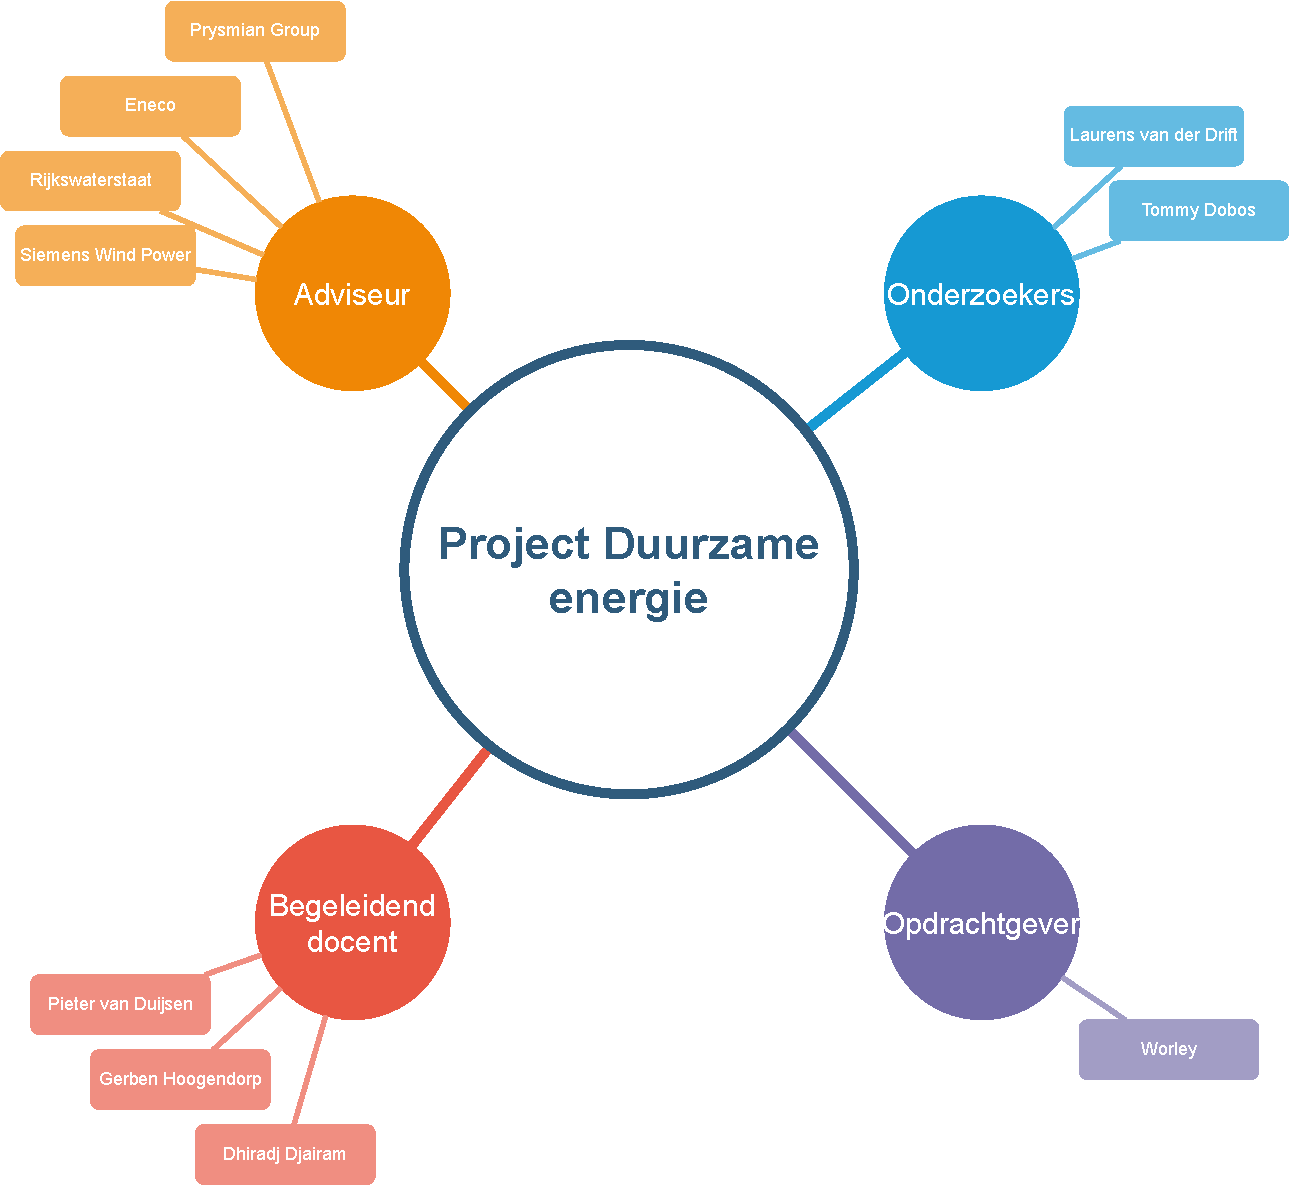
\includepdf[scale=0.65, pages=-]{mindmap/projectorganisatie.pdf}
\end{minipage}